\documentclass{mcmthesis}
\mcmsetup{CTeX = True,   % 使用 CTeX 套装时,设置为 true
        tcn = 83386, problem = A,
        sheet = true, titleinsheet = true, keywordsinsheet = true,
        titlepage = false, abstract = true}
\usepackage{palatino}
\usepackage{lipsum}



\usepackage{url}
\usepackage{hyperref}

%\usepackage[UTF8, nocap]{ctex}

\usepackage{geometry}
%===============设置正文和数学字体=============================
%有些字体需要安装一些字体文件,注意辨别。
%我参照 MCM论文集的字体 使用如下宏包来定制字体。

\usepackage{graphicx}
\usepackage{subfigure}
%设置段落之间的距离,若不需要删除或者注释掉即可。
\setlength\parskip{.5\baselineskip}
\newtheorem{definition}{Definition}[section]
%\def\abstractname{Summary}%可修改摘要名称

\usepackage{indentfirst}
\setlength{\parindent}{2em}

\usepackage{chngpage}
\usepackage{array}
\usepackage{booktabs}
\usepackage{threeparttable}
\usepackage{longtable}
\usepackage[numbers,sort&compress]{natbib}
%%% 实现参考文献标号在右上角
\newcommand{\upcite}[1]%  {\textsuperscript{\textsuperscript{\cite{#1}}}}  原有#
{\textsuperscript{\textsuperscript{\cite{#1}}}}
%然后引用的时候使用\upcite{}的格式(一般的正常引用格式为\cite{})

%\usepackage{cite}      原没有

\usepackage{titletoc}
\titlecontents{section}[3cm]{\bf \large}{\contentslabel{1.8em}}{}{%设置目录标号与文字之间的距离
\titlerule*[0.5pc]{$\cdot$}\contentspage}%
\titlecontents{subsection}[4cm]{\normalsize}{\contentslabel{2.5em}}{}{%
\titlerule*[0.5pc]{$\cdot$}\contentspage}%
\titlecontents{subsubsection}[5.3cm]{\normalsize}{\contentslabel{3.0em}}{}{%
\titlerule*[0.5pc]{$\cdot$}\contentspage}%

\title{\large The Modeling for Ocean's Surface Reflection Radio signals}
\author{ }


\date{\today}

\geometry{left=3.0cm,right=3.0cm}

\begin{document}


\begin{abstract}

In order to solve the practical problems related to the propagation of high frequency shortwave signals on the ocean surface, this paper established the attenuation model of ionospheric reflection signals, this paper also established the reflection model of electromagnetic waves by using the Fresnel reflection coefficient model and its changing formula to study the influence of multi-hop HF radio waves on the ionospheric reflections, whether the waves are turbulent on their reflections, the reflection of terrestrial landforms. It is also meant to study the reflection of hull antennas and the characteristics and environment of propagation in the medium.

Under the condition of known signal transmitting angle and frequency, the mathematic model can find out how many times the multi-hop HF radio can travel back and forth between the ionosphere and the Earth, the losses during propagation and the distance. This paper focuses on the reflection of the ocean surface. When the ocean waves are too large to form a turbulent ocean, the surface reflection problem should be considered as the rough sea surface reflection problem compared with the calm sea surface reflection.

We compare the similarities and differences between the surface reflection contrast of ocean surface and the rugged or flat ground reflection under different environments to analyze the reflection characteristics of different materials under different conditions and also analyze the propagation and losses of HF signals. The antenna receiving gain, wave shaking and receiving weakening should be considerd. Other environmental factors also have a role in signal transmission.




\begin{keywords}
ground reflectio; sea surface reflection; ionosphere;
\\ \hspace*{1.2cm}hull receiving; \hspace*{0cm}nmulti-hop radio shortwave;
\end{keywords}
\end{abstract}
\maketitle
%\pagestyle{empty}
\newpage                                                          %
%==================================================================
%====================生=成=目=录===================================
\begin{adjustwidth}{-1.5cm}{0cm}

\setcounter{tocdepth}{3}
%\thispagestyle{empty}
\tableofcontents                                                  %

\end{adjustwidth}


\newpage

\pagestyle{fancy}

%\setcounter{page}{1}
\section{Introduction}
\subsection{Background}

In the signal transmission, short passes once to the reflection of the ionosphere, and then the first surface reflection in the sea. Depending on the question, we call a process such as ionospheric reflection and a sea surface reflection a jump. In the process of reflection, the ionosphere and the change of the turbulent degree and wave height and wave changes will have a great impact on the reflection. 

Mountain and sea are different, the dielectric constant and the effect of topography on different levels of reflection. We will mountain and ocean analogy correction, make use of the above model in order to study the similarities and differences between the results of the mountain.

\subsection{Analyse of the Problem}

In the signal transmission, short passes once to the reflection of the ionosphere, and then the first surface reflection in the sea. Depending on the question, we call a process such as ionospheric reflection and a sea surface reflection a jump. In the process of reflection, the ionosphere and the change of the turbulent degree and wave height and wave changes will have a great impact on the reflection.


\section{Assumptions}
Taking into account the emphasis of the topic, many factors will affect the accuracy of the model, we make the following assumptions:

\begin{itemize}
\item During the propagation of free space attenuation is 0, and the model in the ideal environment.
\item Short wave reflected by the ionosphere when the ionospheric E layer and the reflection of ionosphere reflection, seemingly level.
\item The launch point from the sea is very near, and by the next ionospheric reflection will be marine reflection.
%%%%%%%%%%%%%%%%%%%%%%%%%%%%%%%%%%%%%%%%%
\end{itemize}

\section{Notations}

\begin{center}
\begin{longtable}{p{.1\textwidth}p{.8\textwidth}m{.4\textwidth}}
\caption{The List of Notation}\\
\hline
Symbol& Meaning \\
\hline

${L_1}$      & Ionospheric absorption decay
                                                         \\
$f$      & The frequency of the transmitted signal
                                                          \\
$f_H$     & The average value of the magnetic rotation frequency at the control point
                                                        \\
$k$       & The number of control points \\
$I_j$      & Absorption coefficient \\
$n$       & Hops \\
$\theta$       & The incident angle \\
$\chi _j$       & The j control points of the solar zenith angle \\
$S_{p12}$       & Sunspot number \\
$R_H$       & The reflection coefficient of horizontal polarization wave \\
$R_V$      & The reflection coefficient of vertical polarized wave \\
$L_g$       & Marine attenuation                      \\
$P$       & The power of the transmitted signal                    \\
$P_{re}$       & Power for the first time after the reflection of calm sea                       \\
$P_n$       & Noise power                                                                \\
$\varepsilon _\gamma$       & The dielectric constant of water                         \\
$N_{max}$       & Ionospheric maximum electron density \\
$f_{max}$       & Maximum frequency                                                     \\
$\rho$       & Correction factor of rough sea surface \\
$R{'_H}$       & The reflection coefficient of horizontal polarization wave correction \\
$R{'_V}$       & The reflection coefficient of vertical polarization wave correction \\
$h$       & The surface RMS height \\
$c$       & Light speed \\
$P{'_{re}}$       & The first time after the reflection of the power of marine Rapids \\
$L{'_g}$       & The modified turbulent ocean absorption attenuation \\
$w$        & Speed of the wind \\
$h$       & Sea level root mean square height \\
$L_{gm}$       & Smooth mountain absorption attenuation \\
${\varepsilon _m}$       & The dielectric constant of the mountain \\
$l_0$       & Signal distance \\
$l{'_0}$       & The actual distance of the signal \\
$\lambda $       & The wavelength of the signal                                                \\
$G_t$       & Antenna gain constant at the source \\
$G_r$       & Receive point antenna gain constant \\
$P_t$       & Transmit power \\
$P_r$       & Receive power \\
$v_c$       & The speed of the boat\\
$t$        & Communication time \\
$d$       & The distance short-wave signal propagation path \\
$f_H$       & The average value of the magnetic rotation frequency at the control point                          \\
${\varepsilon _\gamma }$       & The dielectric constant of sea water                                         \\
%%%%%%%%%%%%%%%%%%%%%%%%%%%%%%%%%%%%%%%%%%%%%%
 \hline
 %\caption{The List of Notation}
 \end{longtable}
 \end{center}




\section{Establishment and solution of the Model}

\subsection{Part 1}
\subsubsection{Analysis of calm waves}


We consider the influence of ionosphere and sea waves tends to calm reflection, and establish the ocean reflectance model based on radio communication, in order to study on the shortwave signal in no less than SNR 10dB, hop shortwave signals.

Take with angle   the reflection of shortwave signal emission as the modeling object, according to the requirements of the subject, in the case of less than MUF, the best emission angle should meet:

\begin{equation} \label{1}
\sin \theta  = \sqrt {1 - \frac{{80.8{N_{\max }}}}{{{f^2}}}}
\end{equation}



\begin{equation} \label{2}
{f_{\max }} = f \times \sec {\theta _{}}
\end{equation}

The first time the reflection of the ionosphere, the ionospheric absorption will be part of the signal, the signal attenuation. We have access to information and by the semi empirical formula commonly used in engineering calculation:%%%%%%%%%%%%%%%%%%%%%%%%%%%%%%%%%%%%%%%%%%%%%%
\begin{equation} \label{3}
{L_1} = \frac{{677.2 \times \sec (\frac{\pi }{2} - \theta )}}{{{{(f + {f_H})}^{1.98}} + 10.2}} \times \frac{1}{k}\sum\limits_{j = 1}^k {{I_j}}
\end{equation}

\begin{equation} \label{4}
{I_j} = (1 + 0.0037{S_{p12}}) \times {(\cos 0.881{\chi _j})^{1.3}}
\end{equation}

Thus, we can calculate ionospheric signal attenuation $L_1$.


From the ionospheric reflection to the sea, the sea is calm, we will process this seemingly specular reflection, but there are still some signal attenuation, we can use the Fresnel reflection coefficient formula:

\begin{equation} \label{5}
{R_H} = \frac{{\sin \theta  - \sqrt {{\varepsilon _\gamma } - {{\cos }^2}\theta } }}{{\sin \theta  + \sqrt {{\varepsilon _\gamma } - {{\cos }^2}\theta } }}
\end{equation}

\begin{equation} \label{6}
{R_V} = \frac{{{\varepsilon _\gamma }\sin \theta  - \sqrt {{\varepsilon _\gamma } - {{\cos }^2}\theta } }}{{{\varepsilon _\gamma }\sin \theta  + \sqrt {{\varepsilon _\gamma } - {{\cos }^2}\theta } }}
\end{equation}

Get the horizontal polarization and vertical polarization wave reflection coefficient by type. Because the signal propagation in strict calculation It is very difficult, we used to deal with such problems in engineering, the incident waves as circular polarized wave, we can use the following formula:

\begin{equation} \label{7}
{L_{\text{g}}}{\text{ = }}10 \times \lg \frac{{{{\left| {{R_V}} \right|}^2} + {{\left| {{R_H}} \right|}^2}}}{2}
\end{equation}

Combination type to calculate the SNR number is less than 10dB before the jump in.

According to the conversion:
\begin{equation} \label{8}
P{\text{ = }}{10^2}W{\text{ = 1}}{{\text{0}}^5}{\text{m}}W{\text{ = }}10\lg {10^{^5}}{\text{d}}B{\text{ = }}50{\text{d}}B
\end{equation}

After the signal strength reflect by calm sea at the first time,  left by following formula:
\begin{equation} \label{9}
{P_{re}} = P - {L_1} - {L_g}
\end{equation}

The title gives us the initial power P constant high frequency carrier signal 100W, and in the calculation of hops before SNR<10dB, a noise signal  . Then, hop it should satisfy the following inequality:
\begin{equation} \label{10}
\frac{{P - n \cdot ({L_1} + {L_g})}}{{{P_n}}} \geqslant 10
\end{equation}

The deformation of inequality:
\begin{equation} \label{11}
n \leqslant \frac{{P - 10{P_n}}}{{{L_1} + {L_g}}}
\end{equation}

The integer part of $n$ is $n_{max}$.

\subsubsection{The Result of the Model}

\begin{table}[!ht]

 \renewcommand\arraystretch{1.5}
 \setlength{\abovecaptionskip}{0pt}%    
\setlength{\belowcaptionskip}{10pt}%
\begin{center}
\begin{tabular}{p{.4\textwidth}p{.4\textwidth}}
\toprule[2pt]
Parameter& Numerical parameters \\
 \midrule

$f$:The transmit frequency signal & $15MHz$ \\

$f_H$:The average value of the magnetic rotation frequency at the control point & $1.5MHz$  \\

$k$:The number of control points & 1  \\

$S_{p12}$:Sunspot number & 1  \\

$P$:The power of the transmitted signal & $100W$  \\

$P_n$:The power of the noise & $1W$  \\

${\varepsilon _\gamma }$:The dielectric constant of water & $80.2Fm^{-1}$  \\

$N_{max}$:For the maximum ionospheric electron density & $50$  \\

 \bottomrule[2pt]
 \end{tabular}
 \end{center} 
 \caption{Datasheets}
 \end{table}
%%%%%%%%%%%%%%%%%%%%%%%%%%%%%%%%
This paper selected control points in a number of reflection point of the ionosphere, we believe in the ionosphere is only one reflection, so $k=1$. The $\theta$ in our model is one of the influencing factors, the $j$ control point in ${\chi _j}$ of the solar zenith angle($j=k=1$), as the complement of $\theta$, The $S_{p12}$ we refer to the sunspot number data from an average of 1$^{\upcite{222}}$, the power of the transmitted signal is $100W$. The noise power $P_n$ we refer to the data set to $1W$, the dielectric constant of water ${\varepsilon _\gamma }$ is about $80.2F{m^{ - 1}}$.

According to equation (1) and (2), we can solve the optimal incident angle $\theta  = {47^ \circ }$.

Using the above formula (3) and (4) for ionospheric absorption and attenuation:
\begin{equation} \label{12}
{L_1} = \frac{{677.2\sec \frac{\pi }{4}}}{{{{(15 + 1.5)}^{1.98}} + 10.2}} \times (1 + 0.0037 \times 1) \times {[\cos (0.881 \times \frac{\pi }{4})]^{1.3}}
\end{equation}

Simultaneous (5), (6) and (7) three attenuation equation can further obtain planar ocean absorption:
\begin{equation} \label{13}
{L_g} =  - 2.0318dB
\end{equation}

According to (8) and the conversion relation formula (9) can power remaining after the first jump to get:
\begin{equation} \label{14}
{P_{re}} = P - {L_1} - {L_g} = 62.8947W
\end{equation}

By (10), (11) formula ${n_{\max }} = 8$. The conclusion is that the maximum jump 8 times.

Therefore, according to this model, the absorption attenuation of high-frequency shortwave through the ionosphere and the absorption attenuation can be calculated after a calm ocean so as to calculate the remaining signal power, and the maximum hops of the high-frequency shortwave reflected by each calm sea surface.


\subsubsection{Waves Stormy Model}

\subsubsection{Analysis of Turbulent Ocean}
Considering the changes in ocean factors impact on the signal too much. We will wave the wave height, wave shape and frequency change and the degree of unity with swift correction factor   rough sea surface is given by the CCIR to consider, the model is improved, which is suitable for the harsh environment of the ocean reflection, namely the ocean situation surging under reflection.

When the water rushing, compared to calm sea, before the first reflection to the surface of the line, using the above equation (1) (2), reflecting on the sea, the situation more complex. We consider the problem is considered as the reflection of the sea rough sea-surface  reflection problem, we introduce the rough correction factor $\rho$:
\begin{equation} \label{15}
R{'_H}{\text{ = }}\rho {R_H}
\end{equation}
\begin{equation} \label{16}
{R_V}'{\text{ = }}\rho {R_V}
\end{equation}

Where:
${R_H}$, $R_V$are smooth in the sea level polarization and vertical polarization wave reflection coefficient.CCIR (International Radio Consultative Committee) the correction factor $\rho$ is express as:
\begin{equation} \label{17}
\rho  = \frac{1}{{\sqrt {3.2g - 2 + \sqrt {{{(3.2g)}^2} - 7g + 9} } }}
\end{equation}

Where:

\begin{equation} \label{18}
g = 0.5{(\frac{{4\pi hf\sin \theta }}{c})^2}
\end{equation}

Here $c$ is the speed of light, $f$ is frequency, $h$ for the surface RMS height, considering the complexity of the $h$ parameter, we introduce Philip Hepburn model:

\begin{equation} \label{19}
h = 0.0051{w^2}
\end{equation}

The same situation is calm ocean waves as incident circularly polarized wave, you can use the following formula:

\begin{equation} \label{20}
{L_g} = 10 \times \lg (\frac{{|R{'_V}{|^2} + |R{'_H}{|^2}}}{{}})
\end{equation}

After the first signal intensity of the rest of the turbulent sea reflection by the following formula:
\begin{equation} \label{21}
P{'_{re}} = P - {L_1} - L{'_g}
\end{equation}

\begin{table}[!ht]

 \renewcommand\arraystretch{1.5}
 \setlength{\abovecaptionskip}{0pt}%    
\setlength{\belowcaptionskip}{10pt}%
\begin{center}
\begin{tabular}{p{.4\textwidth}p{.4\textwidth}}
\toprule[1.8pt]
Parameter& Numerical parameters \\
 \midrule

$c$:Light speed & $3 \times {10^8}m/s$ \\

$f$:Signal transmitting frequency & $15MHz$  \\

$\theta$: The incident angle & ${47^ \circ }$  \\

$w$:Speed of the wind & $25Knot$  \\

 \bottomrule[2pt]
 \end{tabular}
 \end{center} 
 \caption{Datasheets}
 \end{table}

Here we take $c$ as the speed of light $3.0 \times {10^8}m/s$ , $f$, $\theta$ with a value from the best model in the same incident angle, considering the sea breeze is the wind, the wind speed by $w$ is $25Knot$, (3) (4) for ionospheric absorption and attenuation $L_1$ as the same model in (10) results in different places in the turbulent waves when the reflection coefficient is changed by the combination of (15) (16) (17) (18) and the correction factor (19) of the Philip Hepburn model obtained:  

\begin{equation} \label{23}
\rho  = \frac{1}{{\sqrt {3.2g - 2 + \sqrt {{{(3.2g)}^2} - 7g + 9} } }}
\end{equation}

\begin{equation} \label{24}
g = 0.5{(\frac{{4\pi  \cdot 0.0051 \cdot {{25}^2} \cdot 15 \cdot \sin \frac{\pi }{4}}}{{3.0 \times {{10}^8}}})^2}
\end{equation}

\begin{equation} \label{25}
L{'_g} = 10 \times \lg (\frac{{{{\left| {\rho {R_V}} \right|}^2} + {{\left| {\rho {R_H}} \right|}^2}}}{2}) =  - 3.4254dB
\end{equation}

Simultaneous (21) (22) (23) (24) in a combined model $L_1$ whose value can be obtained:

\begin{equation} \label{26}
P{'_{re}} = P - {L_1} - L{'_g} = 45.4414W
\end{equation}

As with calm sea surface, the ionosphere and sea surface absorption attenuation and the residual signal power after the first reflection can be calculated, except that the sea surface absorption attenuation value increases due to the increased complexity of the sea surface.

\subsection{Part 2}

\subsubsection{Analysis of the Problem}

Comparison of the model results mentioned in the rough and smooth degree of mountain with question 1. First consider the smooth mountain, we believe that the smooth region and the sea calm when the state is roughly the same, namely in the first process and before the reflection on the ground are all the same, which led to the first jump of the different residual energy is the process of reflection of the earth and the sea different attenuation, we can use the same model to calculate. So can be compared with mountain and ocean attenuation. But in the calculation is the dielectric constant ${\varepsilon _\gamma }$ changed.

Based on the model 1, we only need a parameter ${\varepsilon _\gamma }$ change into the mountain ${\varepsilon _m }$. You can use the above on the mountain, the smooth model is equation (3) (4) into the following formula:

\begin{equation} \label{27}
{R_{H1}} = \frac{{\sin \theta  - \sqrt {{\varepsilon _{\text{m}}} - {{\cos }^2}\theta } }}{{\sin \theta  + \sqrt {{\varepsilon _{\text{m}}} - {{\cos }^2}\theta } }}
\end{equation}

\begin{equation} \label{28}
{R_{V1}} = \frac{{{\varepsilon _{\text{m}}}\sin \theta  - \sqrt {{\varepsilon _{\text{m}}} - {{\cos }^2}\theta } }}{{{\varepsilon _{\text{m}}}\sin \theta  + \sqrt {{\varepsilon _{\text{m}}} - {{\cos }^2}\theta } }}
\end{equation}

Then the smooth attenuation mountain also increased to that:

\begin{equation} \label{29}
{L_{gm}} = 10 \times \lg (\frac{{{{\left| {{R_{V1}}} \right|}^2} + {{\left| {{R_{H1}}} \right|}^2}}}{2})
\end{equation}

Through access to information found the value of ${\varepsilon _m }$ $15F{m^{ - 1}}$directly, by the formula (26) (27) (28) available:
\begin{equation} \label{30}
{L_{gm}} =  - 4.2093dB
\end{equation}

The rugged mountains are analyzed, in this part, we think that the dielectric constant and the ground is the same, but the difference is that the reflection angle will be affected by the terrain change, and read the data, but could not find the correction factor, the reflection coefficient of the mountain so we consider the angle.

The mountains: a mountain view, assuming the function:$y =  - \frac{1}{4}{x^2} + 8$($ - 4\sqrt {2 < x \leqslant } 4\sqrt 2 $) for the mountains from the upper right to radio model, and the horizontal angle of 45 arrived at the mountain slopes(it $0 \leqslant x \leqslant 4\sqrt 2 $, $0 \leqslant y \leqslant 8$), the slope angle between the horizontal plane and the tangent point is above $k$, $k =  - \frac{1}{2}x$, cotangent function slope, and design $a = |k|$($0 \leqslant a \leqslant 2\sqrt 2 $), in the mountain slopes of the angle of incident radio $\theta$ there are three different situations:

%%%%%%%%%%%%%%%%%%%%Picture%%%%%%%%%%%%%%%%%%%


\begin{itemize}
\item A tangent slope and vertical ratio,$a = 1,\theta  = 0$,
\item The radio arrived at the location in A,$0 \leqslant a \leqslant 1$, $\theta  = \frac{\pi }{4} - \arctan a$,
\item The radio arrived at the location in A, $1 < a \leqslant 2\sqrt 2 $, $\theta  = \arctan a - \frac{\pi }{4}$.
\end{itemize}

The calculated absorption attenuation still (24) (25) (26).

Because the angle is changed, the 1 is invalid, according to 2, 3 wo can get Figure \ref{fig:1} and the $L{'_{gm}}$:

\begin{figure}[htbp]
  \centering
 
  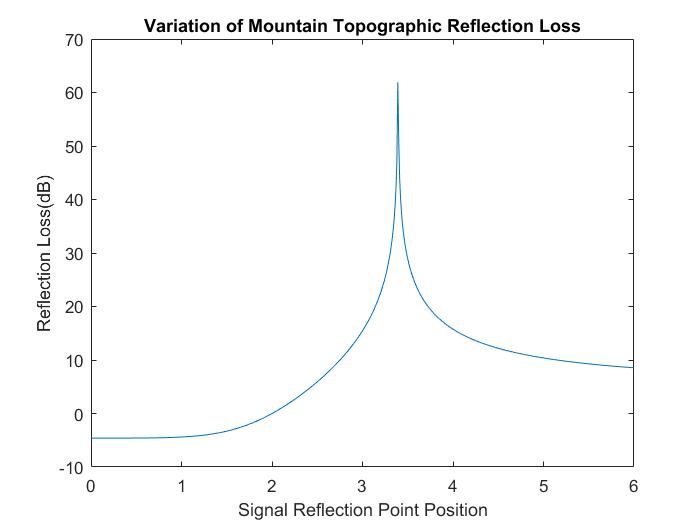
\includegraphics[width=0.7\textwidth]{./picture/plot_2.jpg}
	\caption{}\label{fig:1} 
\end{figure}

\begin{equation} \label{31}
L{'_{gm}} =  - 4.5960dB
\end{equation}

Results: HF in the reflection of mountain and ocean through the mountains and the sea was calm and smooth the analogy, rugged mountainous and rushing sea, found the sea and the mountains, there are the same. By comparing the reflection of the absorption attenuation (13) (20) (29) (30):

\begin{equation} \label{32}
{L_g}{\text{ = }} - 2.0318{\text{dB}}
\end{equation}

\begin{equation} \label{33}
L{'_g} =  - 3.4254dB
\end{equation}

\begin{equation} \label{34}
{L_{{\text{gm}}}}{\text{ = }} - 4.2093{\text{dB  }}
\end{equation}

\begin{equation} \label{35}
L{'_{gm}} =  - 4.5960dB
\end{equation}

\begin{equation} \label{36}
\_\_dB = 10\lg \frac{{{\operatorname{P} _r}}}{{{P_t}}}
\end{equation}


The conclusion can be drawn from the combination of ocean and ocean, mountain and mountain, and ocean and mountain analogy, combined with (31). That is, for ocean and mountainous areas, the relatively smoother reflection surface of the same type of reflection surface absorbs and decays less, and similar results are found after applying the ocean model to the mountain model. But in different smoothness and whether the sea rushing effect on L level is not the same. The reason is that the effect on the ocean, wave reflection and absorption attenuation with many other factors, namely the P. Which factors influence the mountain reflection dielectric constant change. The results show that the smoothing effect of L on whether the sea fast degree will be greater than the mountain of influence to L.


\subsection{Part 3}

\subsubsection{Analysis of the Problem}
First consider how the boat in turbulent ocean better reception issues. Because this part takes into account the raging sea, sailing in the ocean ship reception issues. It takes into account the problem of weather changes, hyperion. We improved on the basis of model two, we added the transmitting and receiving antenna. It will take into account the gain of the antenna and receiving attenuation. Then can calculate the actual power received $P_r$ and the received power of model two $P_{re}$ to compare.

\subsubsection{Improve Model 2}
The boat in the sea to enhance the signal gain of the antenna, it must be considered, is introduced into the model modify:%%%%%%%%%%%%%%%%%%%%%%%%%%%%%%%%%%%
\begin{equation} \label{37}
{l_0} = \sqrt {d_0^2 + ({h_b} - {h_m}^2} 
\end{equation}

\begin{equation} \label{38}
l{'_0} = \sqrt {d_0^2 + {{({h_b} + {h_m})}^2}}
\end{equation}

%\begin{equation} \label{39}
%{p_0}(t) = \sqrt {{G_t}{G_r}} \frac{\lambda }{{4\pi }}(\frac{{{e^{j2\pi {l_0}/\lambda }}}}{{{l_0}}} + \Gamma \frac{{{e^{j2\pi l_0^'/\lambda }}}}{{l_0^'}})
%\end{equation}

Then the formula:
\begin{equation} \label{40}
\frac{{{P_r}}}{{{P_t}}} = \frac{{{G_t}{G_r}{\lambda ^2}}}{{{{(4\pi d)}^2}}}
\end{equation}

(${P_t} = P$, and ${P_r}$, is the power transmission and reception, $G_t$ and $G_r$ are the source point and the receiving point to the antenna gain is calculated according to actual parameters, $\lambda$ is the wavelength of the signal, ${l_0} = d$ is the distance signal, $l{'_0}$ is the actual distance).

Can be calculated $P_r$, $P_{re}$ in the second model, and Compared to what can be found ${P_r} \geqslant {P_{re}}$.

In order to increase muscle response to receive signals, receivers aboard in turbulent ocean travel.

We consider the use of the same multi-hop path, the ship can remain for a long time the problem of communication. The optimal incident angle or with the first ask the same, we still use a reflection model, but because of the waves for non-peaceful state, so the number of hops should be used to calculate the model 2. We need to calculate the signal through the ionosphere to reflect on the sea the most distant (P 0). We assume that the speed of the ship, the calculation using the relationship between the velocity, distance and time:
\begin{equation} \label{41}
P - n({L_1} + L{'_g}) \geqslant 0
\end{equation}

Available:
\begin{equation} \label{42}
n = \frac{P}{{{L_1} + {L_g}}}
\end{equation}

Then use the
\begin{equation} \label{43}
t = \frac{{2nh}}{{{v_c} \times \tan \theta }}
\end{equation}

Get the communication time.

Ionospheric absorption attenuation $L_1$ is the quiet state and non marine attenuation $L{'_g}$. The first question can be calculated directly.P is the start of a given power 100W. The $\theta$ is the optimal incident angle is 47 degrees, ionospheric height $H$, according to data from 110km.

The known amount into the equation $t = 4$. hours. The model is the default for the ship to the shore, so the communication time should be 4 to 11 hours.


\section{The Validate of the Model}
Since the model in this paper has always overlooked one important factor: the decay of free space $L_F$.  The accuracy of this model is greatly reduced. We add this model to the decay $L_F$ of free space so that the model is relatively accurate.

Introduce the commonly used free space loss calculation formula$^{\upcite{444}}$:%%%%%%%%%%%%%%%%%%%%%%%%%%%%%%%%%%%%%%

\begin{equation} \label{44}
{L_F}(dB) = 32.44 + 20 \times \log (f/{f_0}) + 20 \times \log (d/{d_0})
\end{equation}

\begin{equation} \label{45}
{d_0} = 1km
\end{equation}

The $d$ is the short-wave signal propagation path distance, and the $f$ is the frequency of the transmitted signal.

Therefore, in the first question, calculate the calm sea shortwave hops should be ${{\text{n}}_R} \leqslant \frac{{P - 10{P_{\text{n}}}}}{{{L_1} + {L_{\text{g}}} + {L_F}}}$.








\section{Strength and Weaknesses}
\subsection{Strength}
\begin{itemize}
  \item The model compared to other models, the calculation is relatively simple, and close to reality;
  \item The model uses the analogy to study the signal reflection process of the ocean and the mountain, which is useful to popularize;
  \item When studying the complex situation of the ocean, the model is simplified into a correction factor  $\rho$, which is convenient for research.
\end{itemize}

\subsection{Weaknesses}
\begin{itemize}
  \item Compared with the actual life, some parameters of the model are inaccurate, and the error of the calculated results may be larger;
  \item When studying the complex situation in the oceans, we did not take all factors into consideration and considered them quite general;
  \item In the analogy of mountains and oceans, the unique characteristics of mountains and oceans were not used, and the results were inaccurate;
\end{itemize}



\clearpage



\section{A summary of IEEE}
Through the reflection of marine calm surface radio signal model, we can know that the model can be simple and convenient by simultaneous equations calculated according to this model can be calculated by HF ionospheric absorption and attenuation through the calm ocean to absorb the residual signal power, thus calculating the attenuation of high frequency short wave reflection at a time of calm sea surface maximum hop optimal incident angle and number. If the larger waves, sea environment is bad, we can add the rough sea surface is given by CCIR on the basis of the model, the correction factor multiplier P, so that the model can be roughly calculated by HF ionospheric absorption attenuation and attenuation through the complex sea.

Not only that, we can extend it, will change the dielectric constant in the model, to simulate the attenuation calculation of reflection absorption to mountain, sea and mountain, analogy, reflector and similarities. The marine environmental change in the degree of influence on the degree of reflection attenuation is greater than the effect on the smooth degree of mountain mountain reflection attenuation.

The improved model, adding the factor of the gain of the antenna, you can get a new model to enhance the ship in waves is larger on the signal receiving.
This model can calculate the maximum hop frequency shortwave radio is the number on the calm sea. This should be the optimal incident angle, using the angle calculation of ship in turbulent ocean, the maximum number of invalid jump HF power. And with the hop number calculated in the distance can reach the emission signal. According to the actual life in the speed of the ship, it can calculate the ship can remain for a long time communication.



\clearpage

\addcontentsline{toc}{section}{Reference}
\bibliographystyle{plain}
\bibliography{myreference}


\begin{appendices}

\section{First appendix}

Here are simulation programmes we used in our model as follow.\\

\textbf{\textcolor[rgb]{0.98,0.00,0.00}{Input matlab source:}}
\lstinputlisting[language=Matlab]{./code/plot_2.m}

\section{Second appendix}

\textbf{\textcolor[rgb]{0.98,0.00,0.00}{Input Matlab source:}}
\lstinputlisting[language=Matlab]{./code/max_jump.m}

\section{Third appendix}

some more text \textcolor[rgb]{0.98,0.00,0.00}{\textbf{Input Matlab source:}}
\lstinputlisting[language=Matlab]{./code/r_time.m}

\end{appendices}
\end{document}





